% 
% Copyright 2009-2012 Phimeca

%%%%%%%%%%%%%%%%%%%%%%%%%%%%%%%%%%%%%%%%%%%%%%%%%%%%%%%%%%%%%%%%%%%%%%%%%%%%%%%%%%%%%%%%%% 
\section{Architecture guide}

This document makes up the general specification design for the architecture of the Subset module.

\begin{figure}[htb]
  \begin{center}
    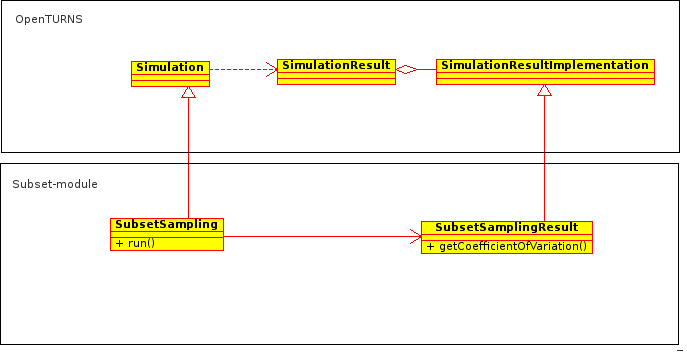
\includegraphics[scale=0.8]{architecture.png}
    \caption{Subset module classes.}\label{fig:architecture}
  \end{center}
\end{figure}


\paragraph{SubsetSampling}

The class SubsetSampling derives from the Simulation class and implements the subset simulation algorithm.\\

\paragraph{SubsetSamplingResult}

The class SubsetSamplingResult derives from SimulationResultImplementation.\\
It allows to store the number of subset steps and return the subset-specific coefficient of variation.\\


